\section{Background} \label{sec:background}

\subsection{KVM} \label{sec:kvm}

KVM is a more recent hypervisor which embeds virtualization capabilities 
in Linux kernel using x86 hardware virtualization extensions~\cite{kivity2007kvm}. 
It is a full virtualization solution, where guests are run unmodified in VMs. It 
consists of two modules, namely, kvm.ko module and an architecture dependent 
kvm-amd.ko or kvm-intel.ko module. Under KVM, each VM is spawned as a regular linux 
process named KVM and scheduled by the default linux scheduler. 

For using shared I/O hardware, these VMs interact with Qemu emulator in host user 
space which provides emulated I/O devices for virtual machines. For instance, in 
the case of network related applications, Qemu provides emulated Network Interface 
Card (NIC) to VMs and interacts with tun-tap device on the other side. The tap device 
is connected to physical NIC through a software bridge.

Figure 1 shows the typical KVM architecture, with reference to a network related
application. 

As depicted in the picture, when a packet arrives at physical NIC,
interrupts generated by NIC are handled by the physical device driver. The device
driver forwards the packet to software bridge. The bridge, then pushes the packet
to the tap device of the corresponding VM. The tap device is a virtual network
device that sends a signal to KVM module. KVM module in turn, generates a virtual
interrupt to the user space Qemu of the target VM. Qemu then copies the packet from
tap device and generates the interrupt for the guest OS emulating the virtual NIC.
Again, the physical device driver in the guest OS handles the packet transfer to
the VM’s address space. A major advantage of the KVM architecture is the full
availability of user-space tools in the QEMU process, such as threading, libraries
and so on.

\begin{figure}[t]
% \vspace{.20in}
\centering
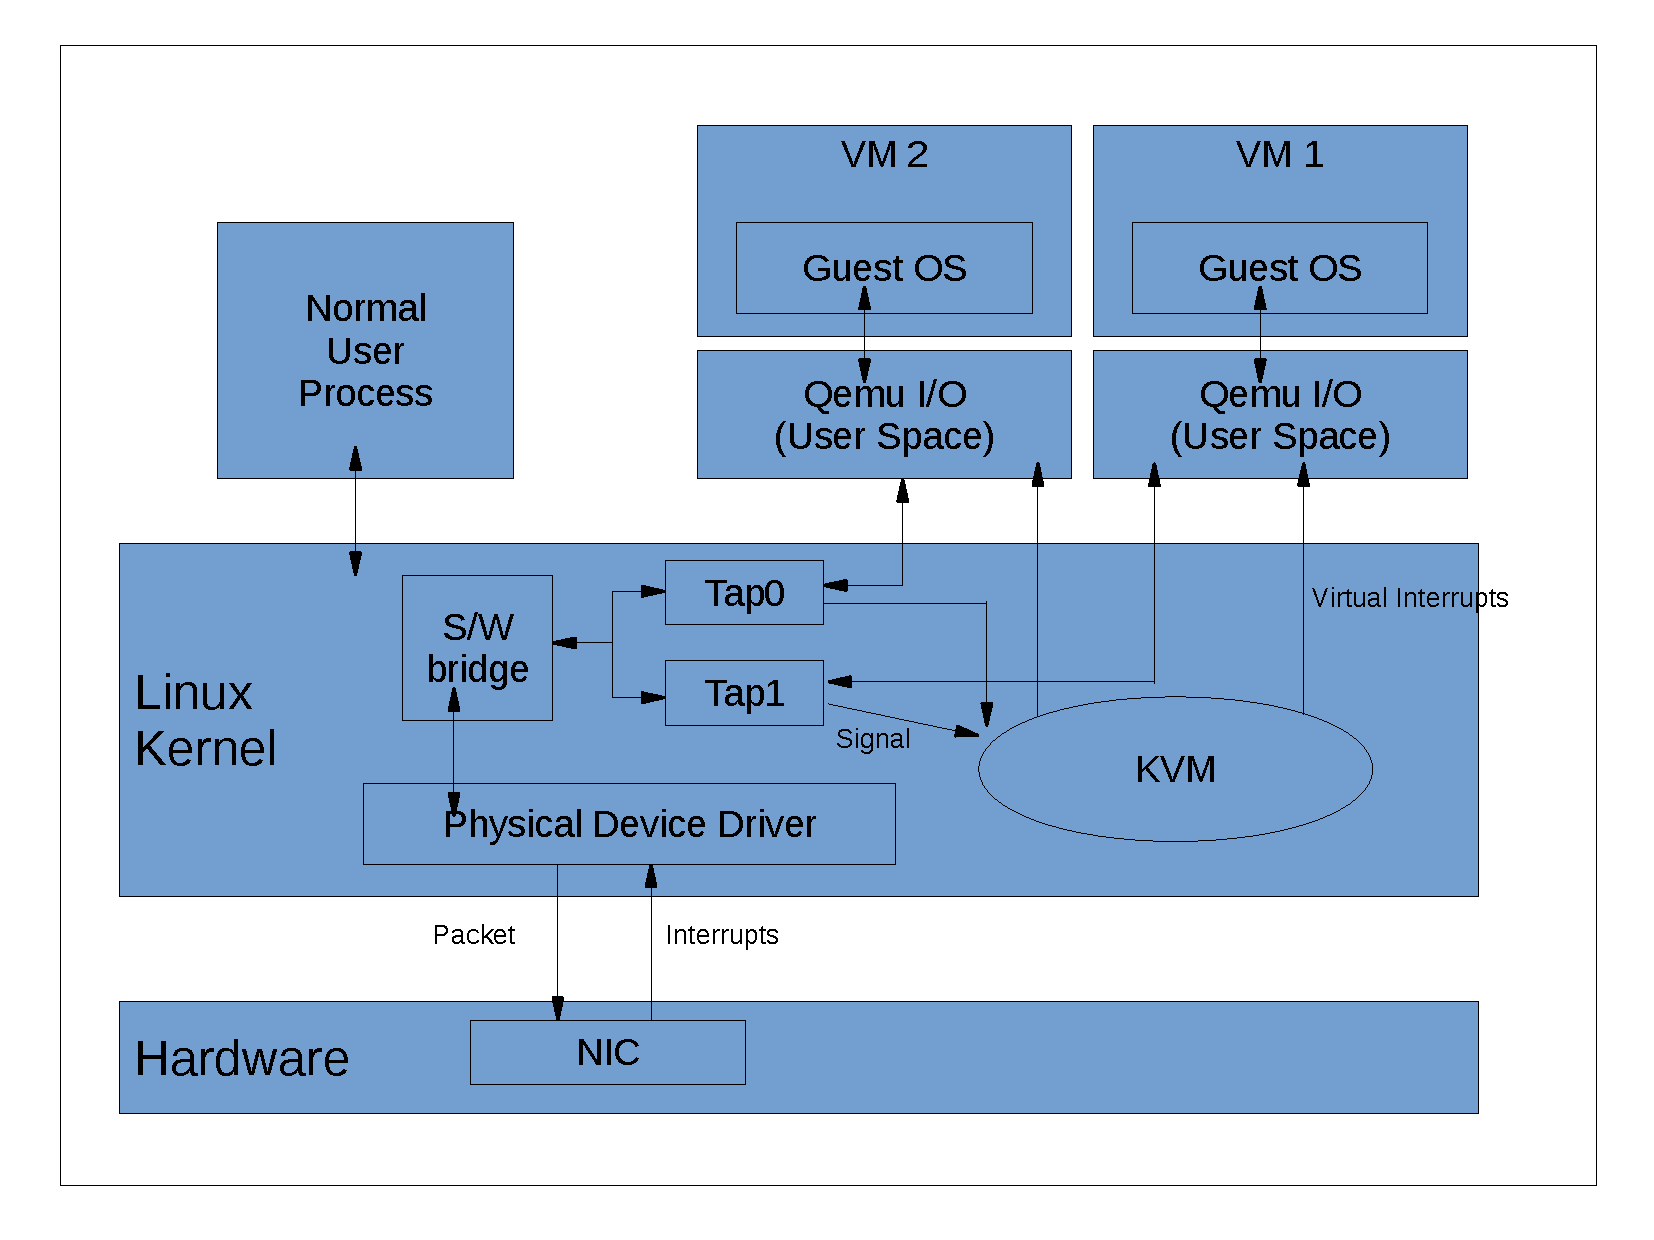
\includegraphics[width=.47\textwidth]{figures/kvm}
\vspace{-.2in}
\caption{{\em KVM Architecture.}} \label{fig:kvm}
\vspace{.05in}
\end{figure}

\subsection{FALCON} \label{sec:falcon}

\smrsystem's deployment model is similar to a typical \smr's. In a \smrsystem-replicated 
system, a set of $2f+1$ machines (nodes) are set up in a InfiniBand cluster. Once the 
\smrsystem system starts, one node becomes the \emph{primary} node which proposes the order of 
requests to execute, and the others become backup nodes which follow the primary’s 
proposals. An arbitrary number of clients in LAN or WAN send network requests to the 
primary and get responses. If failures occur, the nodes run a leader election to elect 
a new leader and continue.

On receiving a client network request, it invokes a RDMA-based consensus process on this 
request to enforce that all replicas see the same sequence of input requests. This process 
has three steps. In the first step, the leader assigns a global, monotonically increasing 
viewstamp to this request, stores this request into an entry that is appended to the consensus 
log, and does a forced write to the local disk. The second step is to replicate the log entry 
on remote servers using a one-sided RDMA Write operation. Usually when the RDMA NIC (RNIC) 
completes the netwrok steps associated with the RDMA operation, it pushes a completion event 
to the queue pair's associated completion queue (CQ) via a DMA write. Using completion events 
adds extra overhead to the RNIC's PCIe bus. Since \paxos could help handle the reliability 
issues, \smrsystem takes advantage of unsignaled RDMA write operations to reduce that overhead, 
i.e., a completion event will not be pushed for these operations. In the last step, the leader 
thread waits for acknowledgments from a majority of nodes.

Unlike previous \smr systems which either reply on deterministic multithreading and replay
approach~\cite{rex:eurosys14} or manually annotate all shared states~\cite{eve:osdi12}, 
\smrsystem deals with nondeterminism at low overhead and automatically. It runs an output 
checking protocol to occasionally detect the inconsistency of the network outputs across replicas. 
If some nodes need to be rolled back, it loads the latest checkpoint. 
